\documentclass{IEEEtran}
\usepackage{mathtools}
\usepackage{graphicx}
\usepackage{amssymb}
\usepackage{amsmath}
\usepackage{pythonhighlight}
\usepackage[utf8]{inputenc}
\usepackage{fancyhdr}
\usepackage{pythonhighlight}
\usepackage{changepage}
\usepackage{slashbox}
\usepackage{floatrow}
\usepackage{listings}
\usepackage[hidelinks]{hyperref}
\usepackage{fontawesome}
\usepackage{caption}
\usepackage{subcaption}
\usepackage[sorting=none,style=ieee]{biblatex}
\addbibresource{report.bib}
\title{Hodgkin and Huxley Cell Membrane Model Simulation}
\author{Kutay Ugurlu}

\begin{document}
\maketitle
\begin{abstract}
    The electrical behaviours of specific kind of organs and structures in human body provide crucial information about the workings of physiological level structures and mechanisms of certain diseases. For diagnosis regarding such structures, many imaging methods have been developed exploiting these behaviors. To do so, a good understanding of the electrical cell behavior is required. This report provides a theoretical background for the action potential behavior, using Hodgkin-Huxley's explanation and explains the methodology to create a simulation software that illustrates the generation and propagation of the action potentials. 
\end{abstract}
\section{Intro}
Hodgkin and Huxley \cite{hodgkin1952quantitative} published a series of five paper in 1952 to explain the generation mechanism of the action potential by introducing their experimental setup and the method. The first paper focused on explaining how the nueron cells work. The second paper investigated the relationship between sodium ion concentration and the membrane voltage, also mentioning the action potential behavior. The third paper examined the effect of sudden conductance changes in the generation of the action potential. It was the fourth paper where Hodgkin and Huxley first explained the sodium inactivation phenomenon. In the last paper, the authors compiled their experimental results and came up with a formulation that explains the action potential generation process. 

\subsection{Voltage Clamp Experiment}

\begin{figure}[h]
\centering
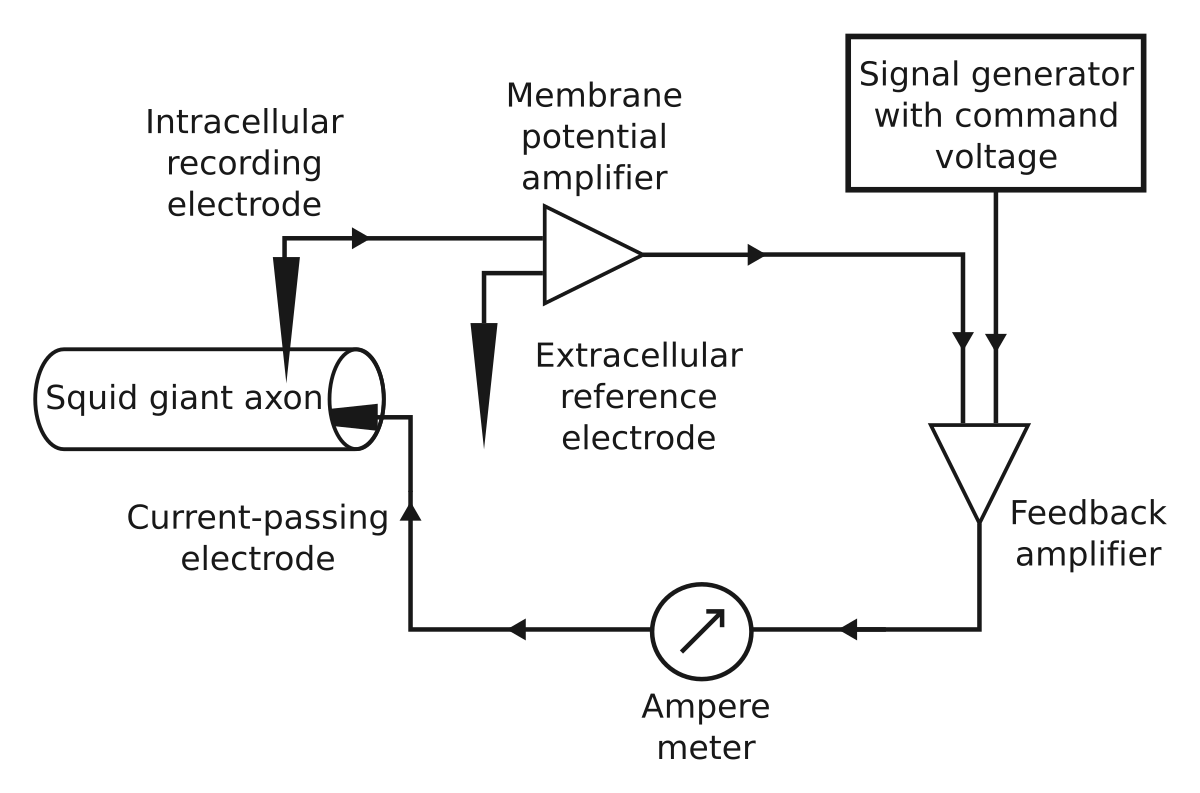
\includegraphics[width=\textwidth]{VCE.png}
\caption{Voltage Clamp Experiment Setup}\label{fig:vce}
\end{figure}

\clearpage
\printbibliography{}
\end{document}

